\section{Kalibrierung des Torsions-Magnetometers}

Die Messwerte der Kalibrierungsmessung sind in Abbildung \ref{fig:MPKalibrierung} zu sehen. Zur Auswertung wird zunächst der durch die Spulen fließende Strom mit dem Spulenkennwert $s$ und der Formel
\begin{equation}
 B=s\cdot I=I\cdot \eb{26,5}{nT}{mA} 
\end{equation}

in das Magnetfeld umgerechnet. Der Plot der Messwerte und der linearen Regression ist in Abbildung \ref{fig:kalibrierung} zu sehen. Bei der Regression ergab sich eine Steigung von $\eb{-0.0039}{Skt}{nT}$. Der negative Kehrwert dieser Steigung liefert den Kalibrierungsfaktor
\begin{equation}
 \frac{\tau}{|\vec{m}|}=\eb{253}{nT}{Skt} \fullstop
\end{equation}

\begin{figure}[!ht]
 \centering
 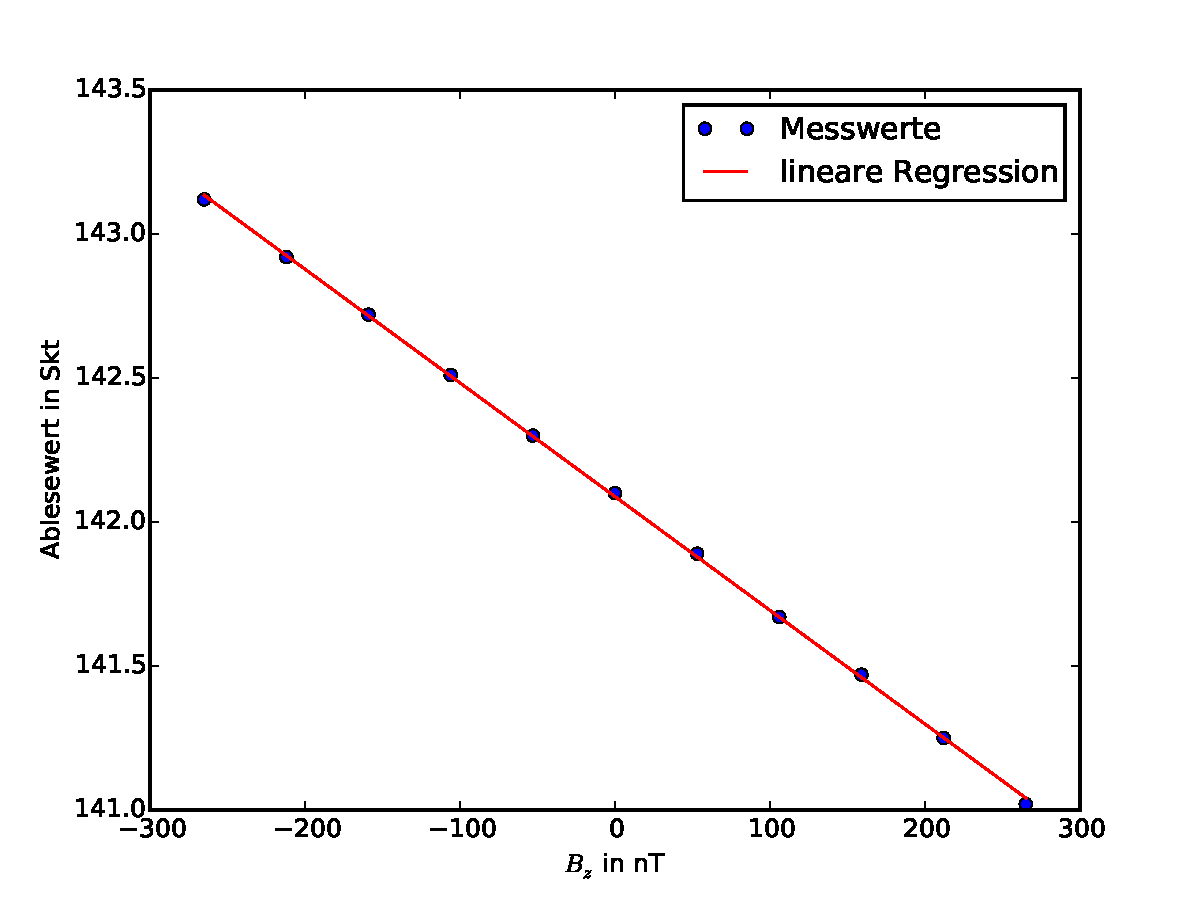
\includegraphics[width=\textwidth]{fig/kalibrierung.pdf}
 \caption[Bestimmung des Kalibrierungsfaktors des Torsions-Magnetometers]{Bestimmung des Kalibrierungsfaktors des Torsions-Magnetometers. Aufgetragen sind die Ablesewerte am Gfz in Skt über die angelegte magnetische Flussdichte in nT.}
 \label{fig:kalibrierung}
\end{figure}

\section{Kartierung}

In Abbildung \ref{fig:Kartierung} ist das Ergebnis der Kartierung abgebildet. Der Basaltgang ist deutlich als magnetische Anomalie zu sehen (in der Abbildung in rot dargestellt). Diese verläuft parallel zur Diagonalen M1-M3. Es bestätigt sich also auch nochmal die Wahl der Lage der Profile entlang von M4-M2 senkrecht zum Gang, die noch genauer untersucht wurden.

\begin{figure}[!ht]
 \centering
 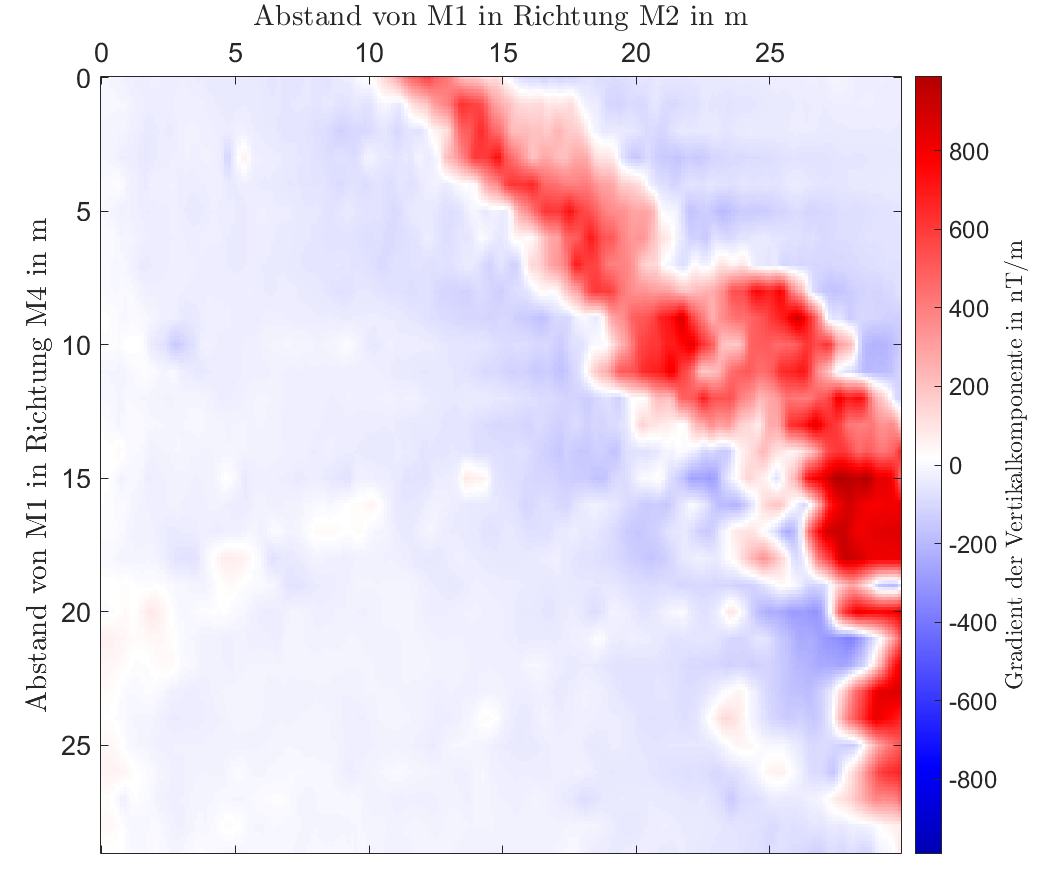
\includegraphics[width=\textwidth]{fig/kartierung_verschwommen.png}
 \caption[Ergebnis der Kartierung]{Ergebnis der Kartierung. M1 befindet sich in der linken oberen Ecke, M2 in der rechten oberen, M3 in der rechten unteren und M4 in der linken unteren.}
 \label{fig:Kartierung}
\end{figure}

\section{Vergleich der Messgeräte}

Das Messprotokoll zum Vergleich der Messgeräte befindet sich in Abbildung \ref{fig:MPVergleich} im Anhang. Die Mittelwerte dieser Messungen stehen in Tabelle \ref{tab:VergleichErgebnis}. Es fällt auf, dass das vom neuen Gerät gemessene Magnetfeld 869\,nT bzw. 897.5\,nT von den anderen Geräten abweicht. Die beiden älteren Protonenmagnetometer weichen mit 28,5\,nT deutlich weniger voneinander ab. Solche kleinen Abweichungen könnten an ungenauen Messungen der Lamorfrequenz liegen, wenn beispielsweise die Beobachtungszeit zu gering war, also nicht genug Periode vermessen wurden. Außerdem könnte die geräteinterne Zeitskala nicht ganz korrekt gewesen sein. Auch die Stangen der Messgeräte hatten vielleicht nicht genau die selbe Länge oder die Messgeräte wurden nicht genau in Richtung Nord-Süd ausgerichtet. Diese Gründe können jedoch vermutlich nicht die größeren Abweichung vom neueren Gerät zu den anderen erklären.

in die Magnetfeldstärke umgerechnet. Der Fehler auf den Strom wird als $\q{\delta}{I}=\e{0,1}{mA}$ angenommen, weil der Wert nur so genau abgelesen werden konnte. Mit Fehlerfortpflanzung ergibt sich daraus der Fehler $\q{\delta}{B}=\e{2,65}{nT}$ auf das Magnetfeld. Der Fehler auf den Ablesewert am Torsions-Magnetometer wird zu $\q{\delta}{\alpha}=\e{0,03}{Skt}$ abgeschätzt, was sich auch aus der Ableseungenauigkeit am Messgerät ergibt. Der Plot der Messwerte mit den eben genannten Fehlern als Fehlerbalken und der linearen Regression ist in Abbildung \ref{fig:kalibrierung} zu sehen. Bei der Regression ergab sich eine Steigung von $\eb{(394,9\pm5,7)\cdot 10^{-5}}{Skt}{nT}$. Der negative Kehrwert dieser Steigung liefert den Kalibrierungsfaktor $k$
\begin{equation}
 k=\frac{\tau}{|\vec{m}|}=\eb{(253\pm3,7)}{nT}{Skt} \comma
\end{equation}
wobei der Fehler aus dem Fehler auf die Steigung mit Fehlerfortpflanzung hervorgeht.

\begin{figure}[!ht]
 \centering
 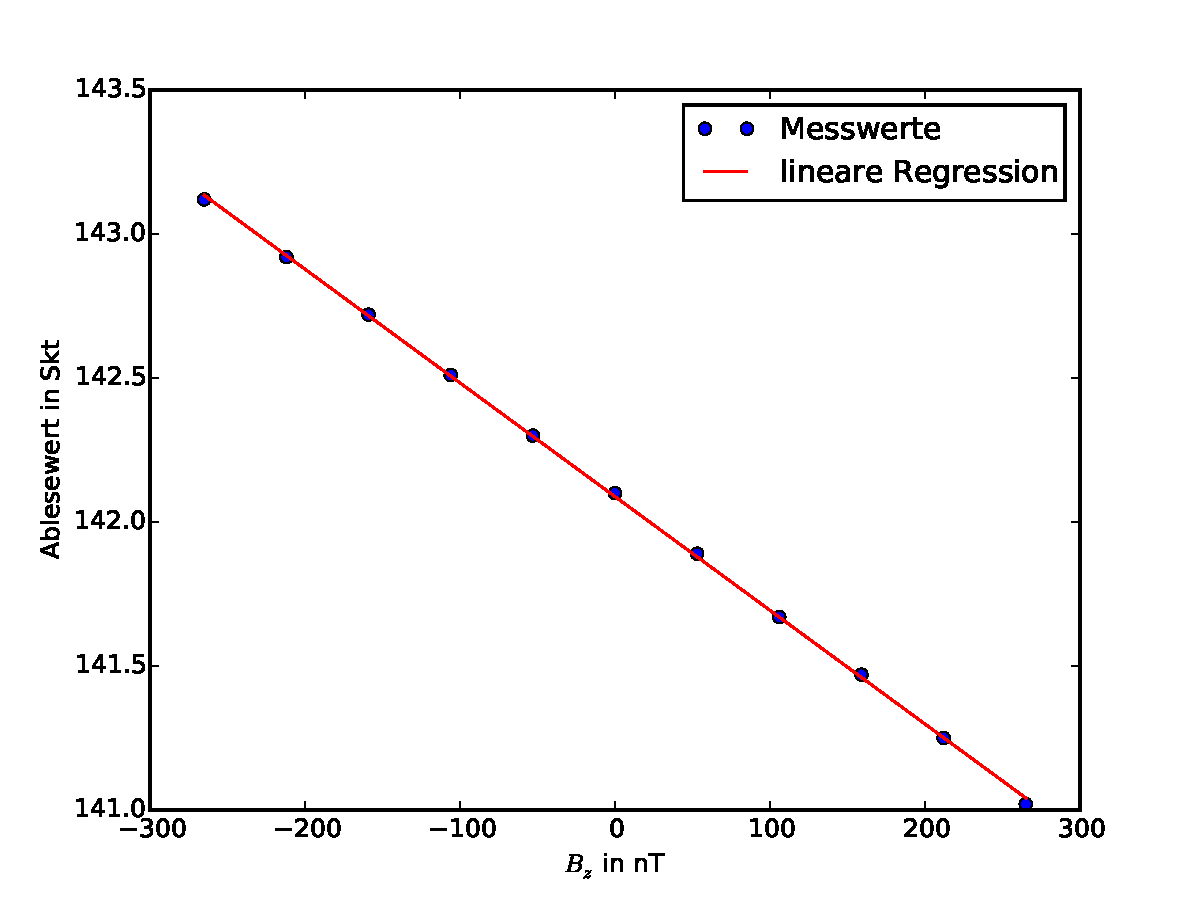
\includegraphics[width=0.8\textwidth]{fig/kalibrierung}
 \caption[Bestimmung des Kalibrierungsfaktors des Torsions-Magnetometers]{Bestimmung des Kalibrierungsfaktors des Torsions-Magnetometers. Aufgetragen sind die Ablesewerte am Gfz in Skt über die angelegte magnetische Flussdichte in nT. Die Fehler sind als Fehlerbalken aufgetragen.}
 \label{fig:kalibrierung}
\end{figure}

\section{Basismessung}

Mit dem Kalibrierungsfaktor können die Werte der Basismessung (siehe Abbildung \ref{fig:MPBasis}) mit Gleichung \eqref{eq:Umrechnung_Torsion} in Einheiten der magnetischen Flussdichte umgerechnet werden. Da die Ruhelage $\alpha_0$ nicht bekannt ist, wird der niedrigste gemessene Wert auf null gesetzt. Man erhält damit also nur Informationen über die zeitliche Änderung des Magnetfelds. 
% Werte mit Fehlerbalken plotten. 
% Auf Laptop schon alle Werte abgetippt?
% tägliche Varianz so gering, dass die Messwerte nicht danach korrigiert werden müssen.

\section{Kartierung}

In Abbildung \ref{fig:Kartierung} ist das Ergebnis der Kartierung abgebildet. Der Basaltgang ist deutlich als magnetische Anomalie zu sehen (in der Abbildung rot dargestellt). Diese verläuft im Bereich der angelegten Profile parallel zur Diagonalen M1-M3. Es bestätigt sich also auch nochmal die Wahl der Lage der Profile entlang von M4-M2 senkrecht zum Gang, die noch genauer untersucht wurden. Abbildung \ref{fig:MagnetikGesamtueberblick} zeigt dies noch einmal genauer. Nur das Profil M26-M27 und das absichtlich schräge Profil M28-M29 sind nicht genau senkrecht über der Anomalie.

\begin{figure}[!ht]
 \centering
 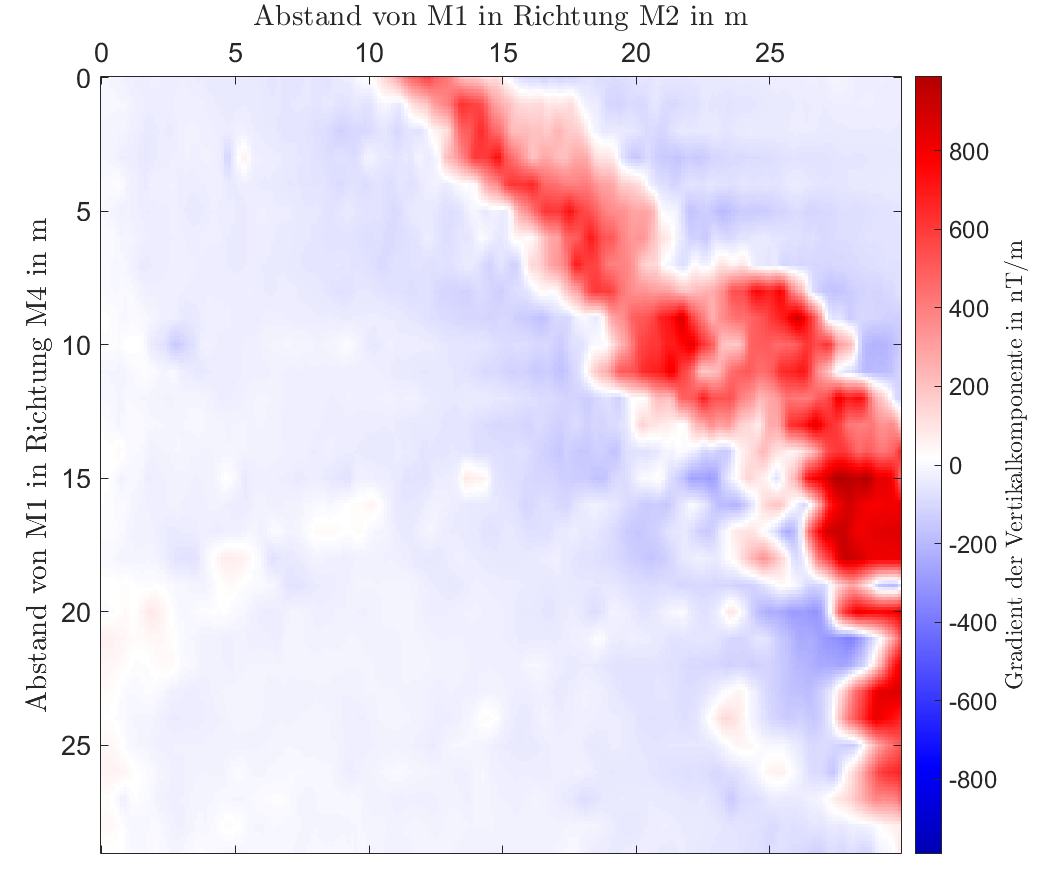
\includegraphics[width=0.8\textwidth]{fig/kartierung_verschwommen.png}
 \caption[Ergebnis der Kartierung]{Ergebnis der Kartierung. Von oben links aus sind die Eckpunkte im Uhrzeigersinn M1, M2, M3 und M4.}
 \label{fig:Kartierung}
\end{figure}

\begin{figure}[!ht]
 \centering
 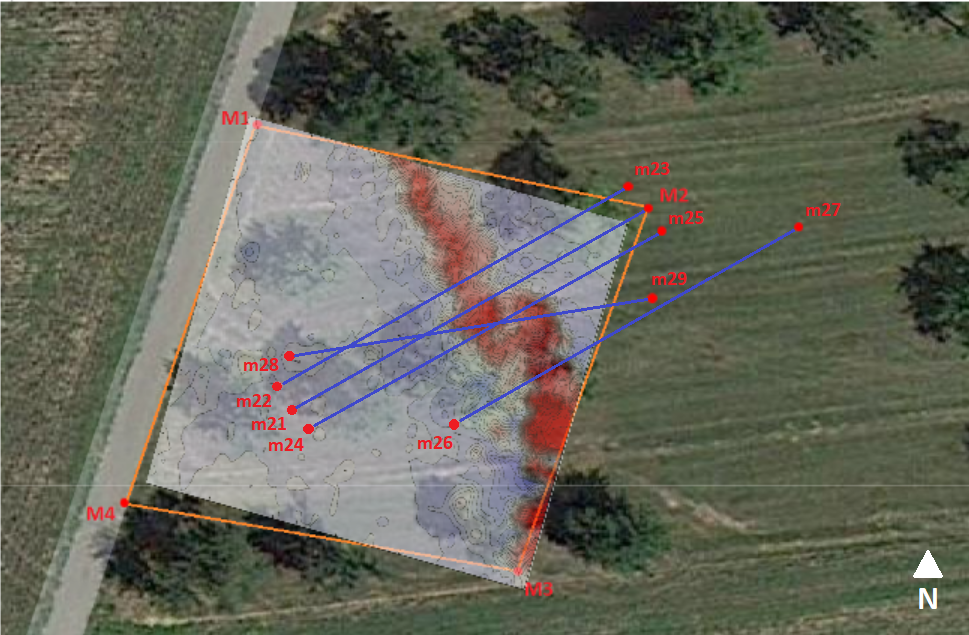
\includegraphics[width=0.8\textwidth]{fig/MagnetikGesamtueberblick}
 \caption[Ergebnis der Kartierung und Lage der der Profile]{Ergebnis der Kartierung und Lage der der Profile. Es ist zu erkennen, dass die drei Profile direkt nebeneinander senkrecht zum Gang verlaufen. M26-M27 ist nicht ganz so gut senkrecht. Die Graphik wurde von Rebekka Kirchgässner und Luisa Rank übernommen.}
 \label{fig:MagnetikGesamtueberblick}
\end{figure}

\section{Vergleich der Messgeräte}

Das Messprotokoll zum Vergleich der Messgeräte befindet sich in Abbildung \ref{fig:MPVergleich} im Anhang. Die Mittelwerte dieser Messungen stehen in Tabelle \ref{tab:VergleichErgebnis}. Es fällt auf, dass das vom neuen Gerät gemessene Magnetfeld 869\,nT bzw. 897.5\,nT von den anderen Geräten abweicht. Die beiden älteren Protonenmagnetometer weichen mit 28,5\,nT deutlich weniger voneinander ab. Solche kleinen Abweichungen könnten an ungenauen Messungen der Lamorfrequenz liegen, wenn beispielsweise die Beobachtungszeit zu gering war, also nicht genug Periode vermessen wurden. Außerdem könnte die geräteinterne Zeitskala nicht ganz korrekt gewesen sein. Auch die Stangen der Messgeräte hatten vielleicht nicht genau die selbe Länge oder die Messgeräte wurden nicht genau in Richtung Nord-Süd ausgerichtet. Diese Gründe können jedoch nicht die größeren Abweichung vom neueren Gerät zu den anderen erklären. Deshalb liegt die Vermutung nahe, dass die Basismessung  mit dem neuen Messgerät fehlerhaft war. Vergleicht man die Messwerte benachbarter Profilendpunkte, weicht das neue Messgerät nicht so stark von den anderen ab wie an der Basisstation.


\begin{table}[!ht]
 \centering
 \caption{Messergebnis des Vergleichs der Protonenmagnetometer und des Fluxgates}

 \begin{tabular}{rl}
 \toprule
 Messgerät & Totalintensität an Basisstation in nT \\
 \midrule
 Nr. 1 & 48102 \\
 Nr. 2 & 48073,5 \\
 Neues Gerät & 48971 \\
 Fluxgate &  \\

 \begin{tabular}{rll}
 \toprule
 Messgerät & Totalintensität an Basisstation in nT & DATASHIFT in nT \\
 \midrule
 Nr. 1 & 48102 &48102\\
 Nr. 2 & 48073,5 & 48073,5\\
 Neues Gerät & 48971 & 48102\\
 Fluxgate & 616,535 & 616,535\\

 \bottomrule
 \end{tabular}
\label{tab:VergleichErgebnis}
\end{table}


Um die Messungen der verschiedenen Messgeräte miteinander vergleichen zu können, muss eines ausgewählt werden, auf das die Messungen mit den anderen korrigiert werden. Dazu verwenden wir die Messungen des Magnetfelds am BFO (siehe Abbildung \ref{fig:BFO}). Aus diesem Diagramm ist abzulesen, dass die Totalintensität des Magnetfelds am BFO am Messtag, den 22.05.2018, von 12:00 Uhr bis 18:00 Uhr zwischen 48220\,nT und 48250\,nT betrug. Die Messwerte des Geräts Nr. 1 liegen am nächsten an diesen, weswegen wir alle Werte auf dieses korrigieren. Es wird also für alle folgenden Auswertungen auf alle Messungen mit Gerät Nr. 2  28,5\,nT addiert und von allen Messungen mit dem neuen Gerät werden 869\,nT subtrahiert.

\section{Profile}

Es wurden 


Um die Messungen der verschiedenen Messgeräte miteinander vergleichen zu können, müssen die Messwerte um ihren jeweiligen Messwert an der Basisstation korrigiert werden. Dies kann im zur Modellierung bereitgestellten MATLAB-Skript im DATASHIFT realisiert werden. Bei den anderen Plots, die noch folgen, wurde diese Korrektur auch durchgeführt. Für das neue Messgerät wurde der gleiche DATASHIFT wie für Nr. 1 verwendet, weil die sonstigen Messwerte dieser beiden Geräte am nächsten aneinander liegen und die Messung an der Basisstation vom neuen Gerät aufgrund ihrer Falschheit nicht verwendet werden kann.

% Fehlerhaft und alt:
% Um die Messungen der verschiedenen Messgeräte miteinander vergleichen zu können, muss eines ausgewählt werden, auf das die Messungen mit den anderen korrigiert werden. Dazu verwenden wir die Messungen des Magnetfelds am BFO (siehe Abbildung \ref{fig:BFO}). Aus diesem Diagramm ist abzulesen, dass die Totalintensität des Magnetfelds am BFO am Messtag, den 22.05.2018, von 12:00 Uhr bis 18:00 Uhr zwischen 48220\,nT und 48250\,nT betrug. Die Messwerte des Geräts Nr. 1 liegen am nächsten an diesen, weswegen wir alle Werte auf dieses korrigieren. Es wird also für alle folgenden Auswertungen auf alle Messungen mit Gerät Nr. 2  28,5\,nT addiert und von allen Messungen mit dem neuen Gerät werden 869\,nT subtrahiert. In den Modellierungen mit Matlab kann dies dadurch erreicht werden, dass bei allen Geräten der Messwert des ersten Messgeräts an der Basisstation als DATASHIFT verwendet wird.

\section{Profile}

Im folgenden werden die vermessenen Profile ausgewertet. Die Messprotokolle befinden sich im Anhang in den Abbildungen \ref{fig:MPProfil_erstes} bis \ref{fig:MPProfil_letztes}. Sie werden qualitativ verglichen und manche werden mit dem bereitgestellten MATLAB-Skript modelliert.

%Erklärung Parameter Modellierung
Bei der Modellierung mit MATLAB werden einige Parameter per Hand eingegeben und dann die Anomalie mit diesen Parametern berechnet. Die Messwerte und berechneten Werten können dann verglichen werden und ein möglichst gut die Werte erklärendes Modell gefunden werden. Die Inklination $\q{I}{H}=63,75^\circ$ und Totalintensität $\q{T}{H}=\e{48000}{nT}$ des Hintergrundfelds waren bereits gesetzt und wurden auch nicht verändert, da sie in der kurzen Zeitskala der Versuche gleich bleiben. Der DATASHIFT wurde wie oben beschrieben geräteabhängig eingestellt. Der Streichwinkel das Gangs wurde mit Grafik \ref{fig:MagnetikGesamtueberblick} aus der Kartierung bestimmt. Dies ist der Einkel abgetragen im Gegenuhrzeigersinn zwischen Nord-Süd-Richtung und Gang. Er wurde mit einem Geodreieck als 29$^\circ$ gemessen. Die magnetische Suszeptibilität von Basalt scheint in einem sehr großen Bereich zu liegen, was es schwierig machte, diese festzulegen. Der Default-Wert 0,015 wurde zu 0,017 geändert, weil so die Modellierungen allgemein etwas besser wurden. Die Tiefe der Gangunterkante wurde mit 1000\,m sehr tief gesetzt, weil der Gang als magnetische Anomalie in einer uns zur Verfügung gestellten geologischen Karte eingezeichnet war. Er verlief auch durch einen Schnitt und reichte bezüglich der Tiefe durch den ganzen Schnitt hindurch. Die Position des Maximums der gemessenen Werte wurde profilabhängig anhand der Messdaten eingestellt und und die Länge der Stange der Protonenmagnetometer ist bei allen drei 2\,m. Da diese Werte bei allen Modellierungen so gesetzt wurden, kann nur noch die Neigung des Gangs, die Tiefe der Gangoberkante und die Gangbreite verändert werden.
%%So schreiben ???:
Dies schränkt die Möglichkeiten der Modelle zwar ein, ist aber eigentlich nicht wirklich gerechtfertigt, weil nicht genau und unbefriedigend begründet werden kann, warum die gerade aufgelisteten Parameter so gesetzt wurden.

%%Modellierung mit Kati und Niels zusammen erwähnen!!!

\subsection{Profile M22-M23, M21-M2 und M24-M25}

Diese Profile haben einen Abstand von 2\,m zueinander und sind nach der Kartierung zu schließen senkrecht zum Gang. Es ist also anzunehmen, dass die Messwerte abzüglich der Vergleichsmessung an der Basisstation sehr ähnlich verlaufen sollten. In Abbildung \ref{fig:Vergleich_Profile} ist dies zu sehen. Es fällt auf, dass die Totalintensitäten nach Süden hin zunehmen. Unter der Annahme, dass die magnetische Suszeptibilität des Gangs, sein Streichwinkel und seine Neigung gleich bleiben, würde dies dafür sprechen, dass er beim südlichsten Profil näher an der Erdoberfläche ist. Diese These wird durch das MATLAB-Modellierungsskript unterstützt. Lässt man alle Parameter unverändert und verkleinert nur die Tiefe der Gangoberkante, nehmen die berechneten Totalintensitäten über der Anomalie zu. Außerdem wird das Maximum nach Süden hin breiter, was vermuten lässt, dass der Gang in diese Richtung breiter wird.

Im folgenden wird ein Modell beschrieben, bei dem nur wenige Parameter geändert werden müssen, um für alle drei Profile eine möglichst kleine Abweichung von den Messwerten zu erhalten.

\begin{figure}
 \centering
 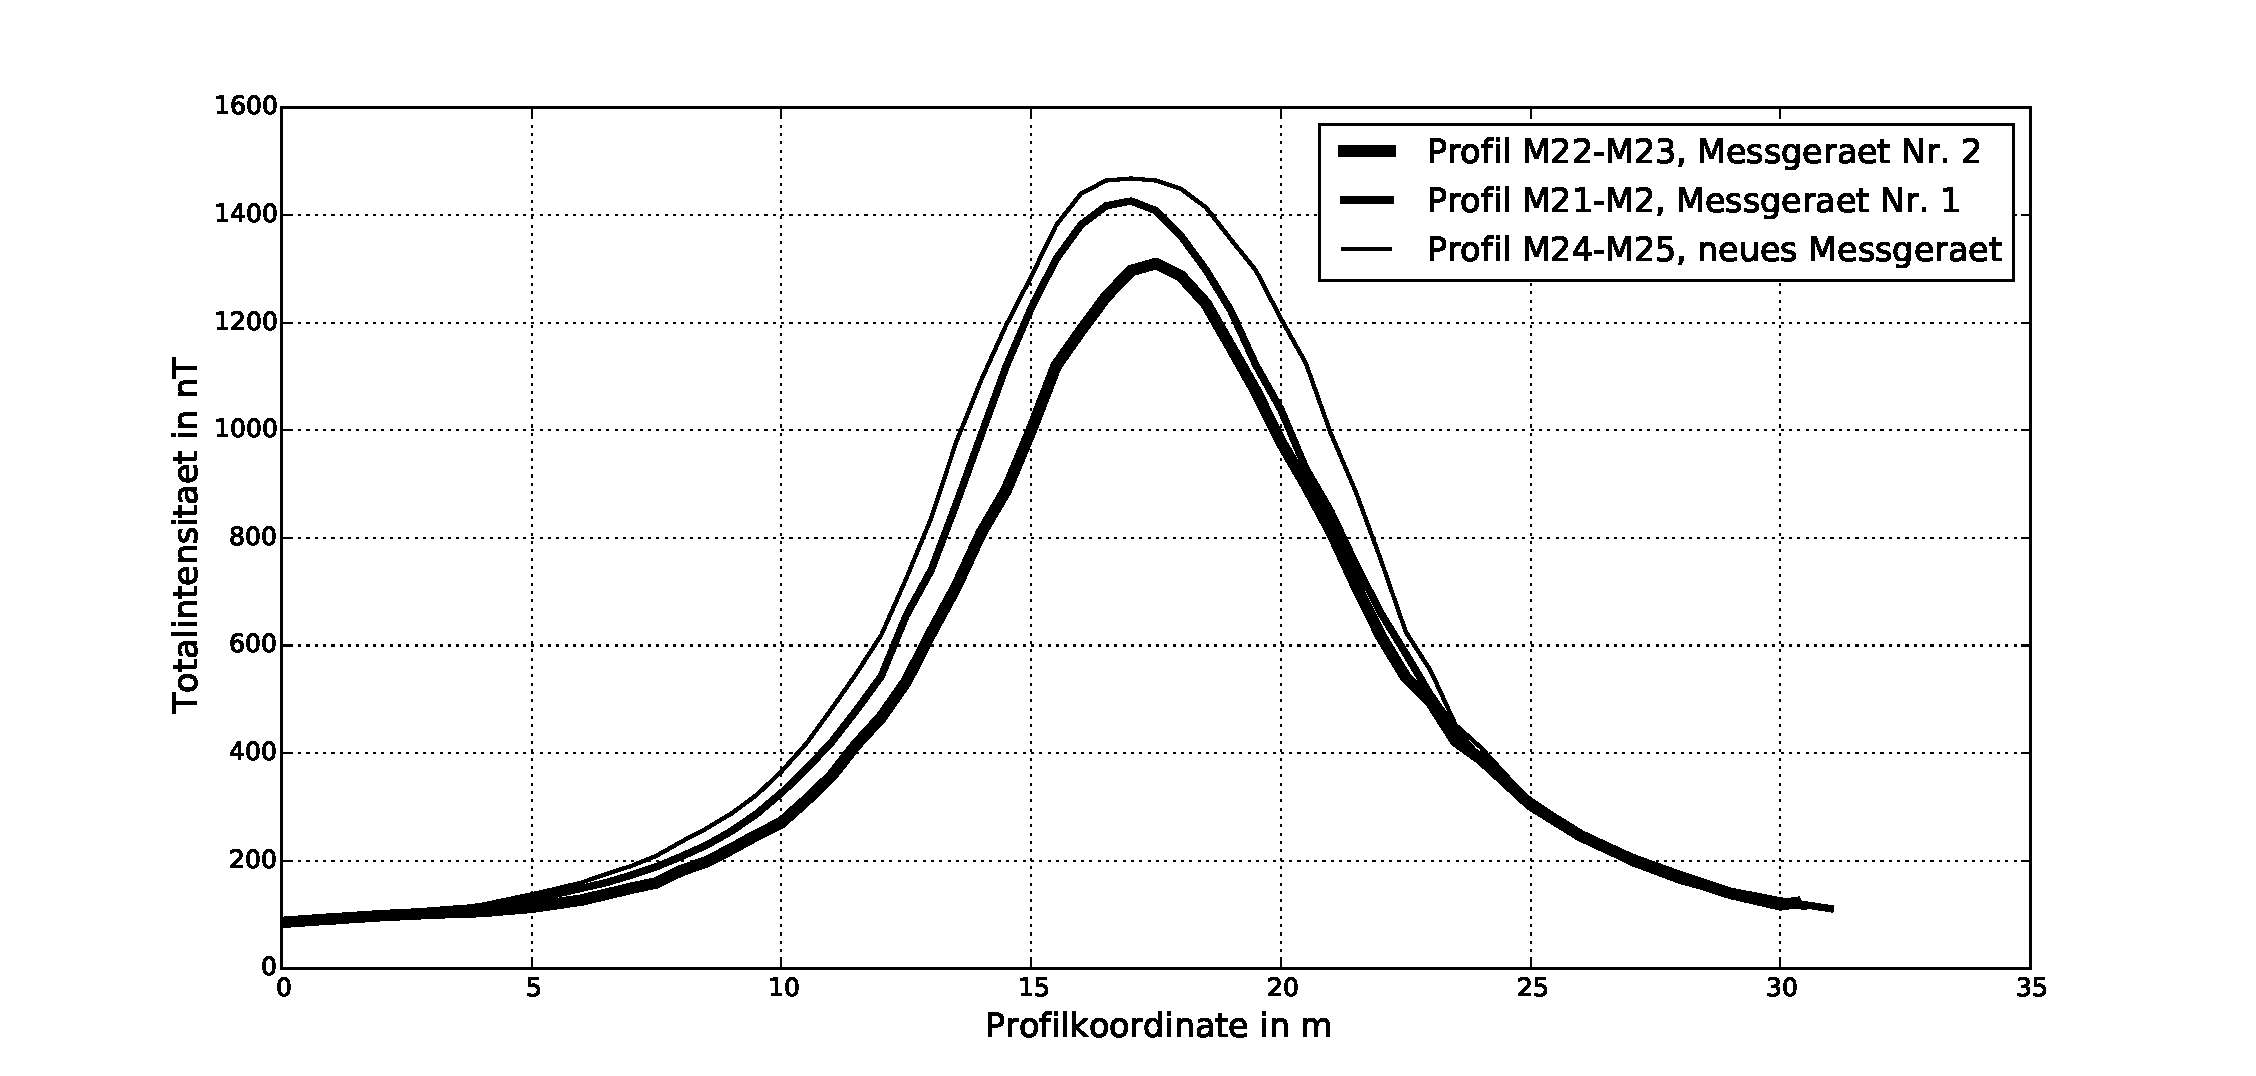
\includegraphics[width=\textwidth]{fig/Vergleich_nahe_Profile.pdf}
 \caption[Vergleich der Profile M22-M23, M21-M2 und M24-M25]{Vergleich der Profile M22-M23, M21-M2 und M24-M25. Die Profilkoordinate ist jeweils vom erstgenannten Profilende aus gemessen und die Messwerte wurden bereits mit der Vergleichsmessung normiert.}
 \label{fig:Vergleich_Profile}
\end{figure}

\subsubsection{Profil M22-M23}

Eine mögliche Modellierung für dieses Profil ist in Abbildung \ref{fig:modM22} zu sehen. Es fällt auf, dass das Modell abwechselnd über und unter den Messwerten liegt. Bei der Durchführung der Modellierung fiel auf, dass dies durch eine Änderung des Streichwinkels beseitigt werden könnte. Da dieser aber der einzige Parameter ist, der durch die Kartierung genau bekannt ist, wurde dies nicht gemacht. Stattdessen wurde die Neigung des Gang geändert. Bei einem Winkel von 16$^\circ$ zur Senkrechten passte das Modell am besten zu den Messwerten. Durch diesen Parameter kann die Form der Messwerte jedoch nicht exakt wiedergegeben werden. Die Breite und Tiefe der Gangoberkante wurden so variiert, dass der Verlauf am Maximum wie bei den Messwerten aussieht.

\begin{figure}
 \centering
 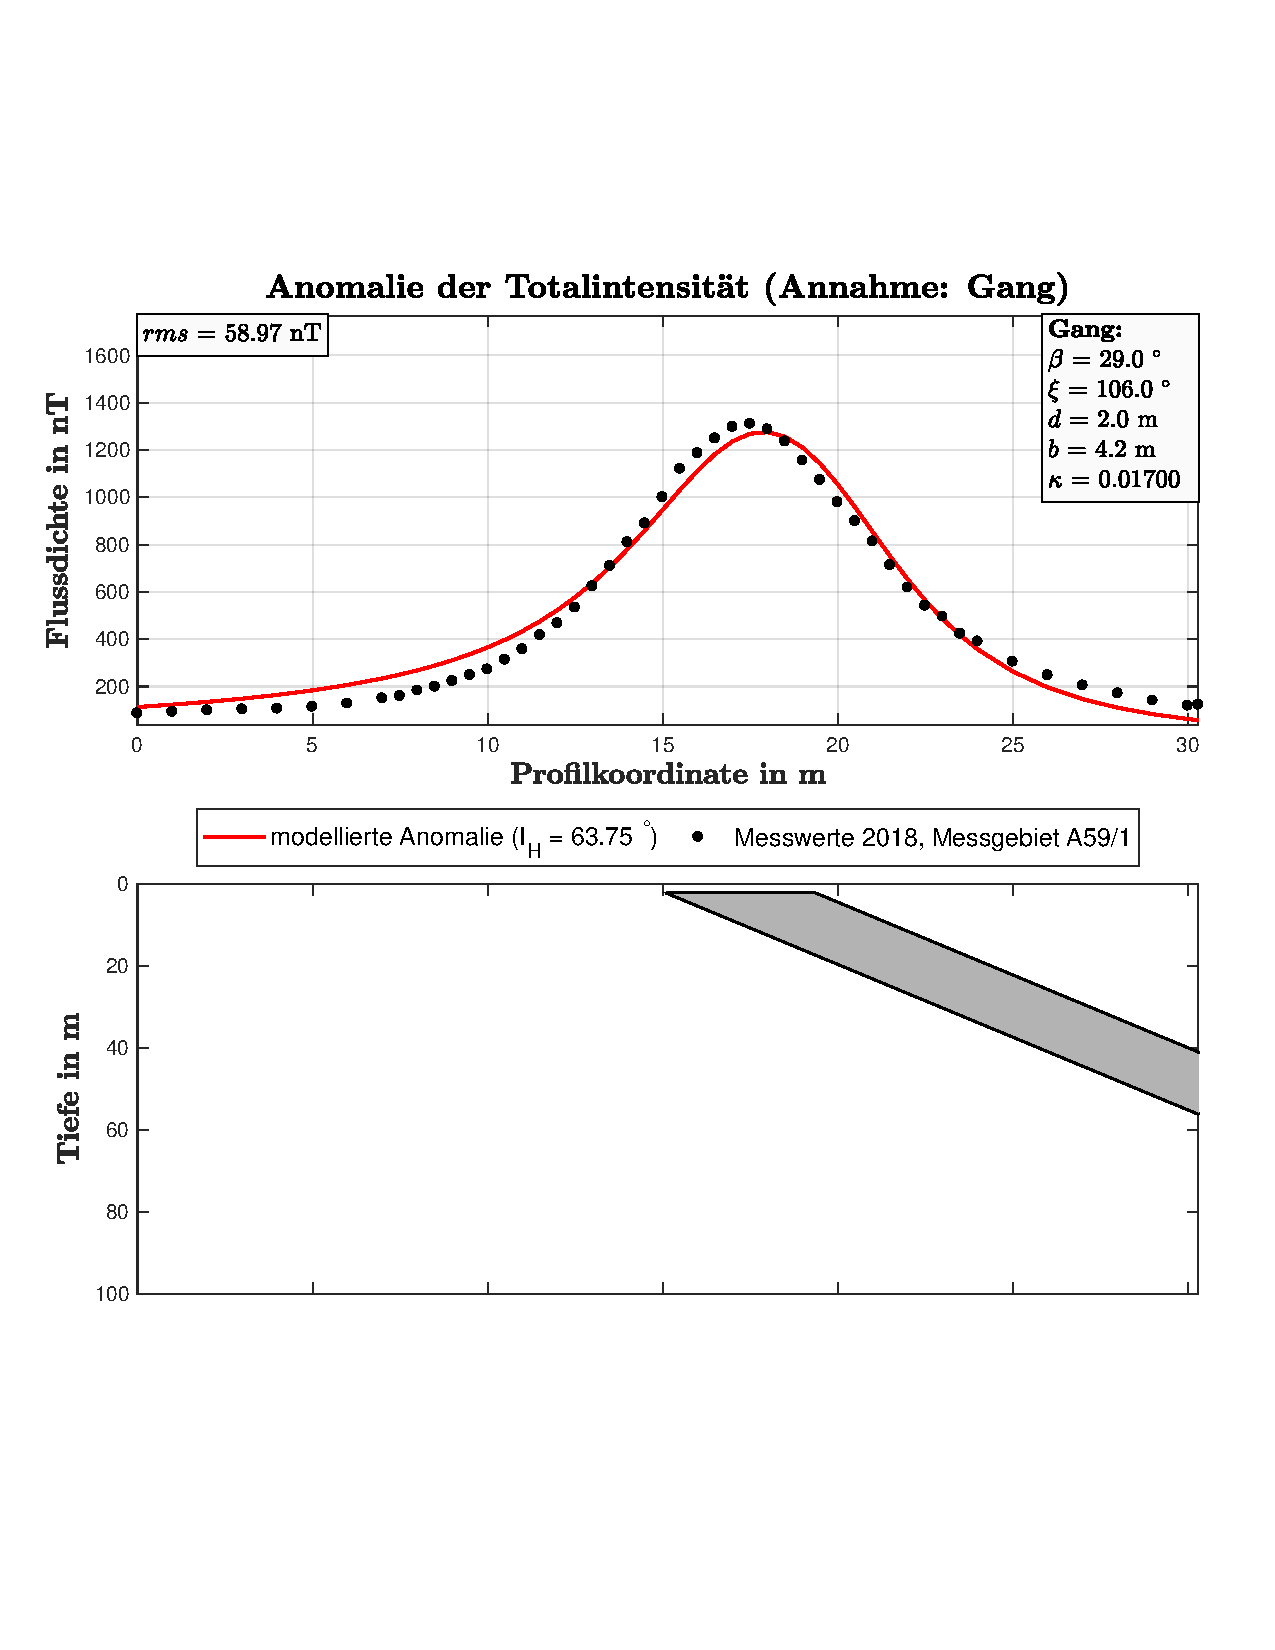
\includegraphics[width=\textwidth]{fig/modM22}
 \caption{MATLAB-Modellierung des Profils M22-M23}
 \label{fig:modM22}
\end{figure}

\subsubsection{Profil M21-M2}

Die Modellierung dieses Profils ist in Abbildung \ref{fig:modM21} dargestellt. Auch bei diesem Profil hätte der Streichwinkel geändert werden müssen, um die Modellierung besser zu den Messergebissen passen lassen zu können. Die Neigung konnte im Vergleich zu Profil M22-M23 gleich bleiben und nur die Tiefe und Breite des Gang wurden verändert. Er ist an dieser Stelle vermutlich 20\,cm breiter und befindet sich 40\,cm näher an der Erdoberfläche. Dadurch können die oben genannten Vermutungen bestätigt werden.

\begin{figure}
 \centering
 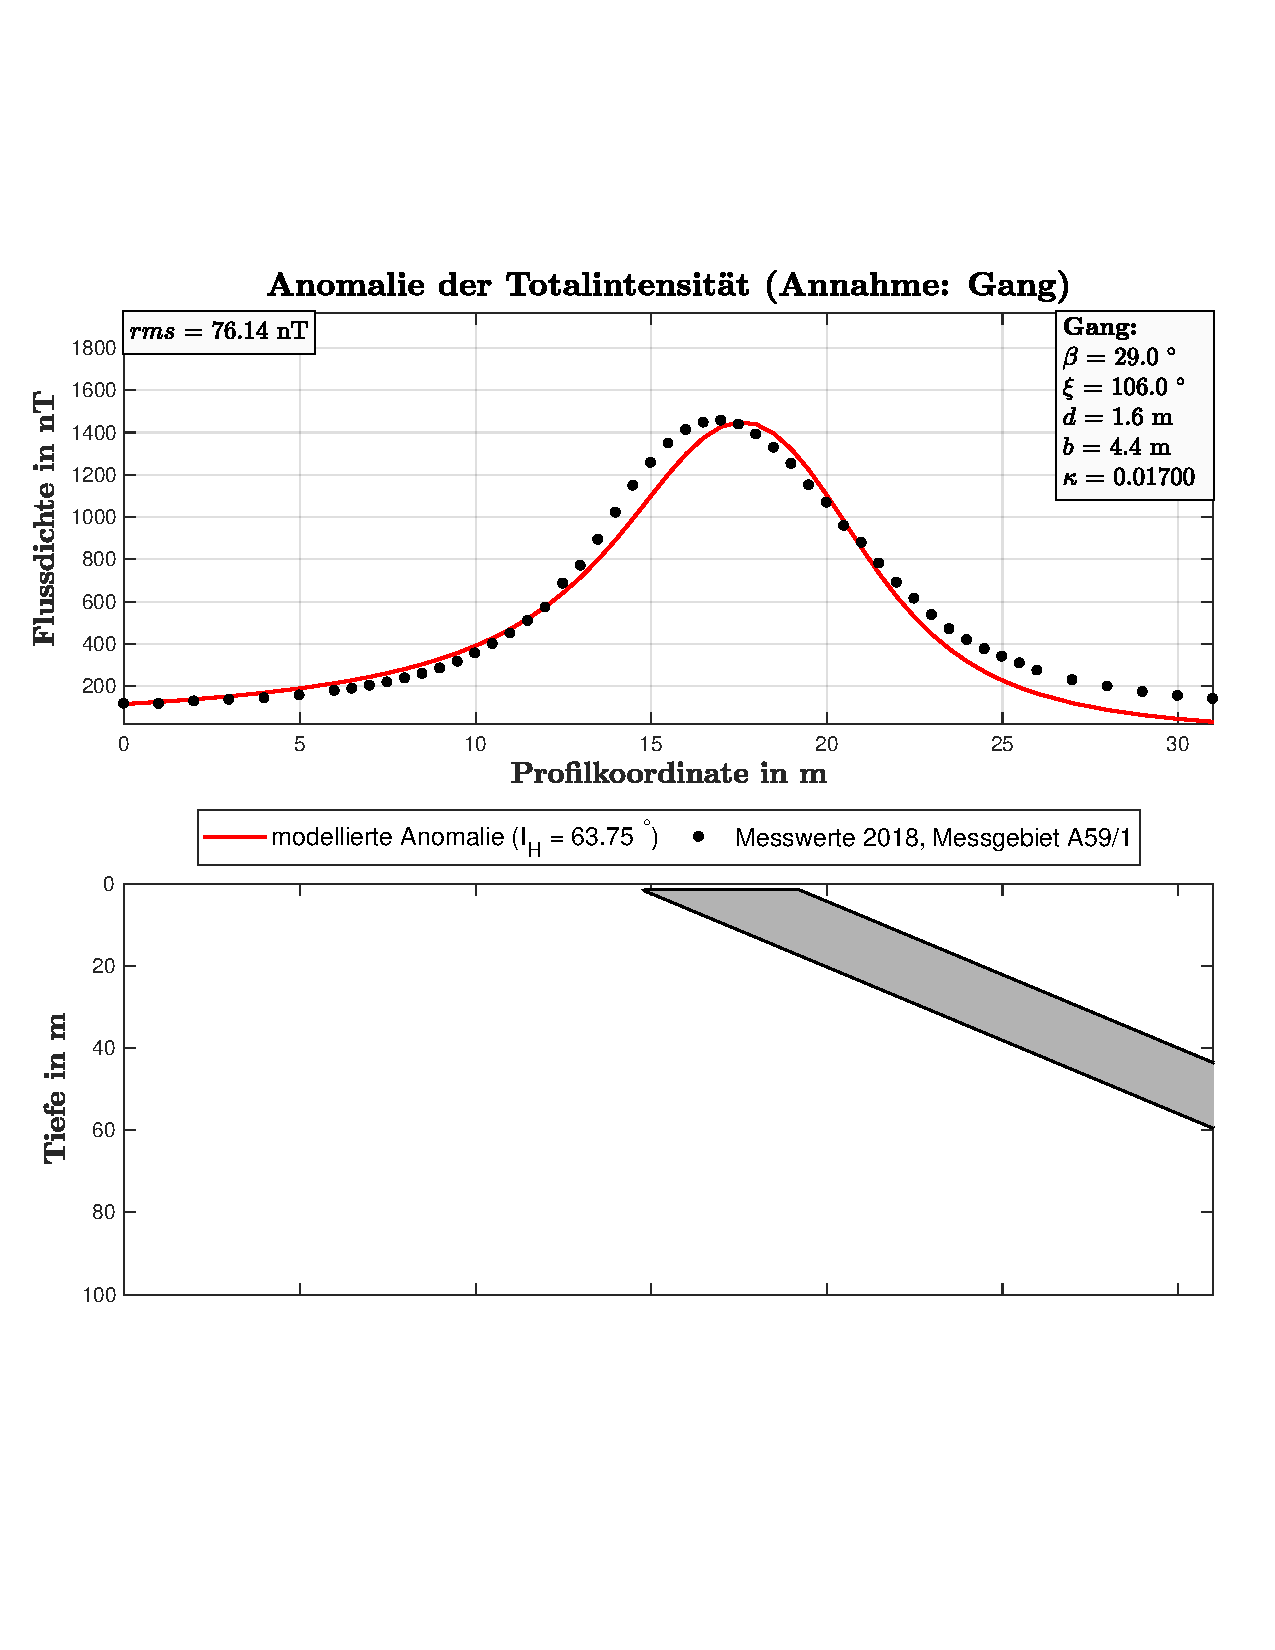
\includegraphics[width=\textwidth]{fig/modM21}
 \caption{MATLAB-Modellierung des Profils M21-M2}
 \label{fig:modM21}
\end{figure}

\subsubsection{Profil M24-M25}

Die Modellierung dieses Profils ist in Abbildung \ref{fig:modM24}. Das Maximum wird noch breiter als bei den schon beschriebenen Modellen. Deswegen wurde die Gangbreite noch einmal 30\,cm vergrößert. 

\begin{figure}
 \centering
 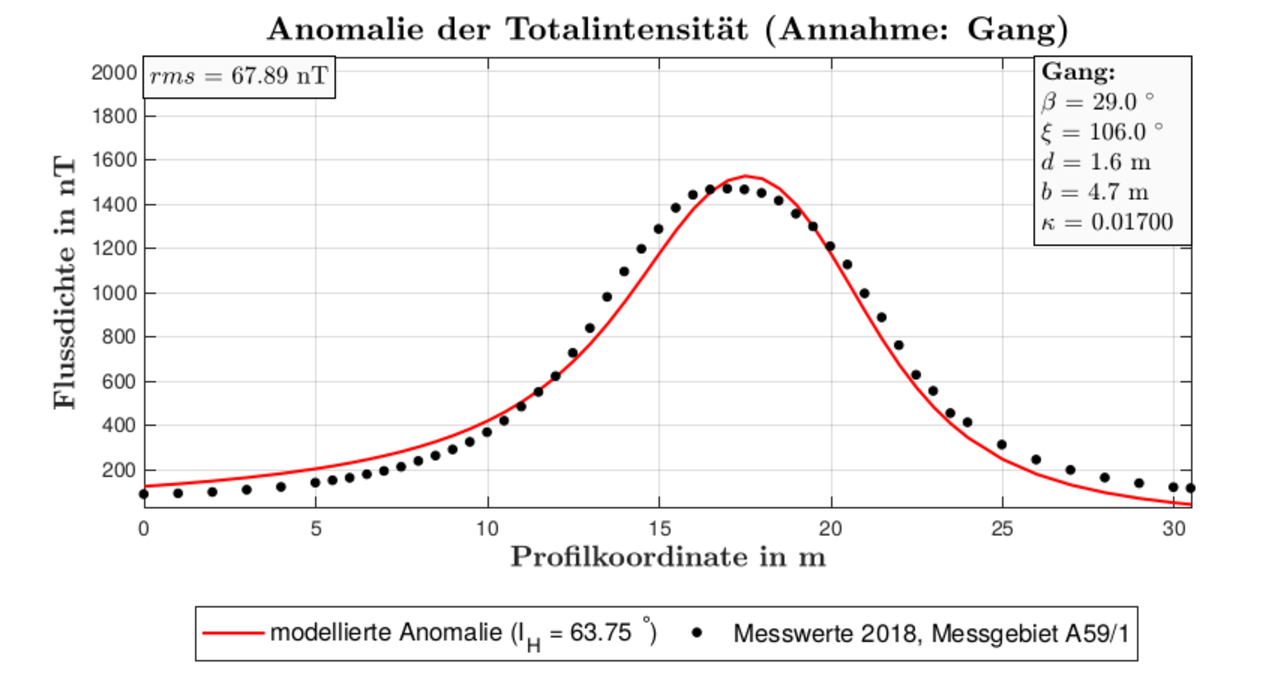
\includegraphics[width=\textwidth]{fig/modM24}
 \caption{MATLAB-Modellierung des Profils M24-M25}
 \label{fig:modM24}
\end{figure}


\subsection{Profil M26-M27}

Dieses Profli ist parallel zu M24-M25 in einem Abstand von 5\,m angelegt. Da es weiter östlich beginnt, befindet es sich nicht mittig über dem Basaltgang. Wie in Abbildung \ref{fig:modM26} ist deswegen nur nur der rechte Ausläufer der Anomalie vermessen worden. Im Vergleich zu Profil M24-M25 wurde in der Modellierung nur die Neigung geändert, um die Messwerte zu beschreiben. Im Bereich des Maximums stimmen Modellierung und Beobachtung gut überein. Nur am Ausläufer ist das Modell unter den den Messwerten. Dies ist nicht sehr verwunderlich, weil die Modellierung immer 15\,m bis 20\,m neben dem Maximum bereits gegen Null geht und dies bei unseren Messungen nicht der Fall ist, weil wir als DATASHIFT den Messwert an der Basisstation verwenden und nicht den niedrigsten auf dem Profil gemessenen Wert.

\begin{figure}
 \centering
 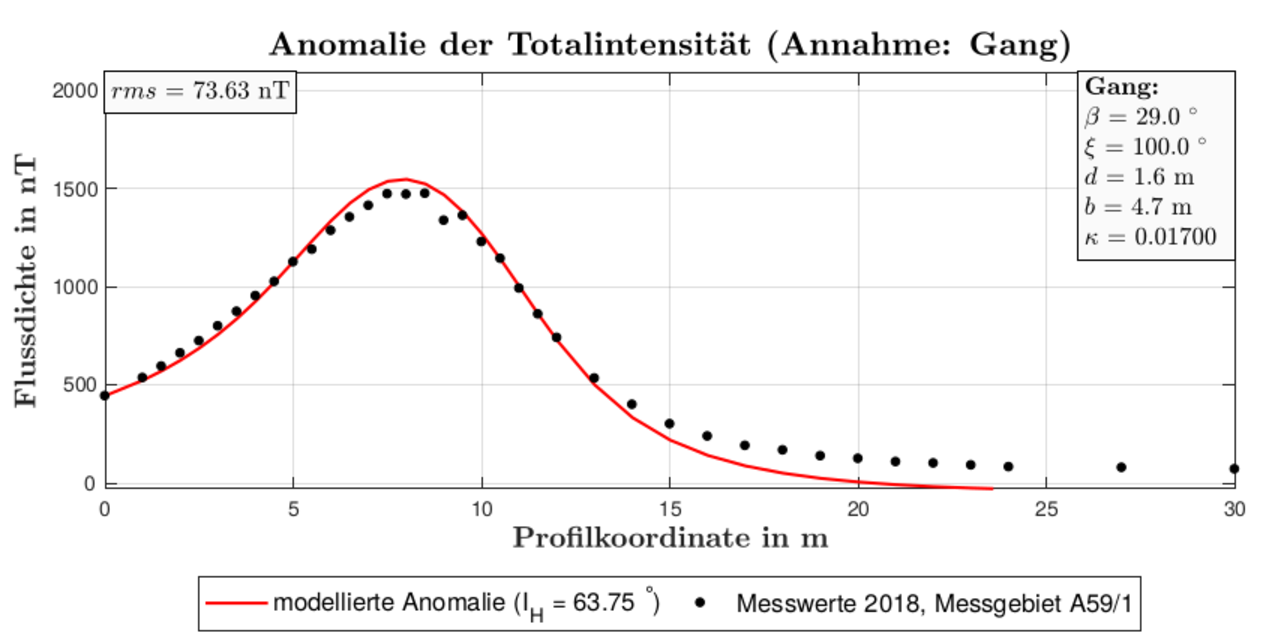
\includegraphics[width=\textwidth]{fig/modM26}
 \caption{MATLAB-Modellierung des Profils M26-M27}
 \label{fig:modM26}
\end{figure}

\subsection{Profil M28-M29}

Dieses Profil ist nicht senkrecht zum Gang angelegt. In der Mitte des Gangs befindet es sich an der gleichen Stelle über diesem wie Profil M24-M25. Deswegen ist in Abbildung \ref{fig:modM28} die Modellierung mit genau den gleichen Parametern wie bei Profil M24-M25 durchgeführt. Diese Modellierung erklärt die Messergebnisse nicht gut, weil durch die schräge Lage das Maximum viel breiter ist als bei den anderen Profilen. Um diese breite Kurve modellieren zu können, müsste zum Beispiel die magnetische Suszeptibilität sehr viel größer gewählt werden.

\begin{figure}
 \centering
 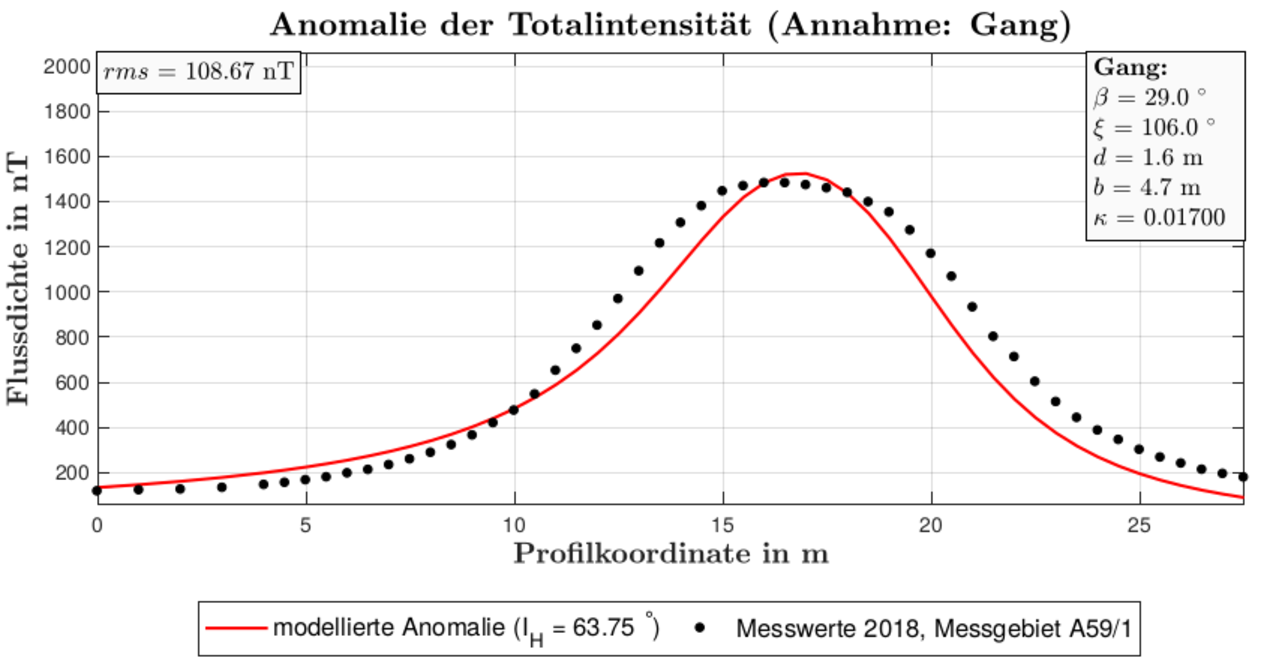
\includegraphics[width=\textwidth]{fig/modM28}
 \caption{MATLAB-Modellierung des Profils M28-M29}
 \label{fig:modM28}
\end{figure}


% \begin{figure}
%  \centering
%  \includegraphics[width=\textwidth]{fig/}
%  \caption{}
%  \label{fig:}
% \end{figure}